%%=============================================================================
%% Conclusie
%%=============================================================================

\chapter{Discussion}
\label{ch:conclusie}

Quantum computing will most definitely become one of the great buzzwords of the next decade. With the release of Google's paper around their interpretation of 'Quantum supremacy', the whole field was catapulted to the forefront of research. All the big players in Quantum research have been given a tremendous spotlight for the future of profitable quantum computing. And this is precisely why we need to make the whole concept more approachable for anybody interested.

\subsection{Quantum computing for now}

From the research around the subject, there are a couple of interesting conclusions to draw. Beginning with one of the most important ones, Quantum computing is here to stay. The technology has proven too much promise in too many sectors that have a strong financial backbone. Think about fields like medicine, where they analyse their drugs in such small dimensions that even those observations have their own quantum effects that could interfere with the effect of drugs as whole on the human body. At this point it is important to understand that the world around us that is visible with the naked eye is completely homogeneous with the 'quantum world', meaning that all research to exploring our world around is can only be profitable towards the future.

To return back to the more concrete conclusions of this paper. While executing this specific version of Grover's algorithm, there was a clear trend visible between the theory and the practical example that does show there are some growing pains that come with the expansion of our quantum devices.
Yes, the theory can be fully implemented at this point to visualise its results when we would work in the most perfect of environments like a simulator. But this perfect environment simply does not exist in the real world or at least for now it doesn't. Meaning that we will have to be creative to reach this edge of perfect conditions to get to a point that these simulated algorithms can become reliable and profitable towards the future. There are 2 ways of trying to fix the issue of quantum decoherence. The first would be to actually create devices that are not influenced by any internal/ external interferences that could provide a stable platform for algorithms like Shor's encryption breaking algorithm. The other option would be to account for these interferences to happen anyway and try and compensate against them in a software way, much in the same way a computer does error correction for downloaded files. The latter seems to be the more reasonable option where we are already trying to implement these quantum error correction in to provide better results. For now there is no clear technique behind the whole principle except to play around with the length that a qubit needs to stay in its elevated $\ket{1}$ state and the length of the circuit as a whole

But this all can be tried out, because at the moment of writing we are able to extensively experiment with real or simulated quantum devices. There is a multitude of platforms available, where most of them are open-source and you are free to contribute to them as you want to expand their feature-set. Frameworks like Qiskit allow you to design quantum circuits and test them using their built in simulators, which are easy to pick up and hard to master. As of now IBMQ is the only service that allows you to push up your circuits to really test them on a real device owned and managed by IBM. By granting people the privilege to pay around with the real devices and notice the shortcomings through raw data results, really shows off how dedicated the whole community of computer science is on pushing this technology to the forefront.


\subsection{Quantum computing and its myths}

As shown in the experiment, QC will not break our entire world in the next decade in any drastic manner. So theories that quantum computing could break our entire encryption standard in a matter of years seem absurd once you look at the real executions of these needed algorithms on real quantum devices.
Nevertheless we do want to work proactively to have solutions ready-to-go once these machines do become powerful enough to brute force the RSA-encryption by finding the factors of the prime numbers that represent the private keys of encrypted files.
There is also the notion that quantum decoherence will prove to have an insurmountable mountain the more qubits we start adding to the systems. This indeed is a major hurdle that needs to be overcome to make quantum computing the new standard for solving really hard to solve problems in the computer science community.

\subsection{Quantum computing as an addition}

The one thing we should take away from the dawn of quantum computing the following decade, is that quantum computing is not the one solution for every single issue in computing. It has its advantages and disadvantages just like classical computing. We should strive to make these 2 technologies as complementary as possible so that they can cancel out each others disadvantages and amplify their advantages respectively. 

With this work, we have tried to inspire people to learn more about the subject of quantum computing and to hopefully entice them into writing their own 'Hello-world-Applications' on any of the freely available frameworks.

\subsection{Future works}

As to conclude back with the main subject of this paper, the potential powerhouse of a mainframe device and a quantum computer. If IBM keeps up it doubling pace of releasing quantum computational resources into the world each year and the quantum error correction evolves to an acceptable percentage, we could start thinking about implementing QC machine learning in our mainframes or even the speeding up the database structures in the devices. But for now QC and mainframe are not able to cooperate in an useful manner to give back business value. 

It is good to explore these options upfront so that we know when the time comes to expand QC towards the mainframe we have a clear scope to all the potential applications of these 2 devices.


\begin{figure}[h]
	\centering
	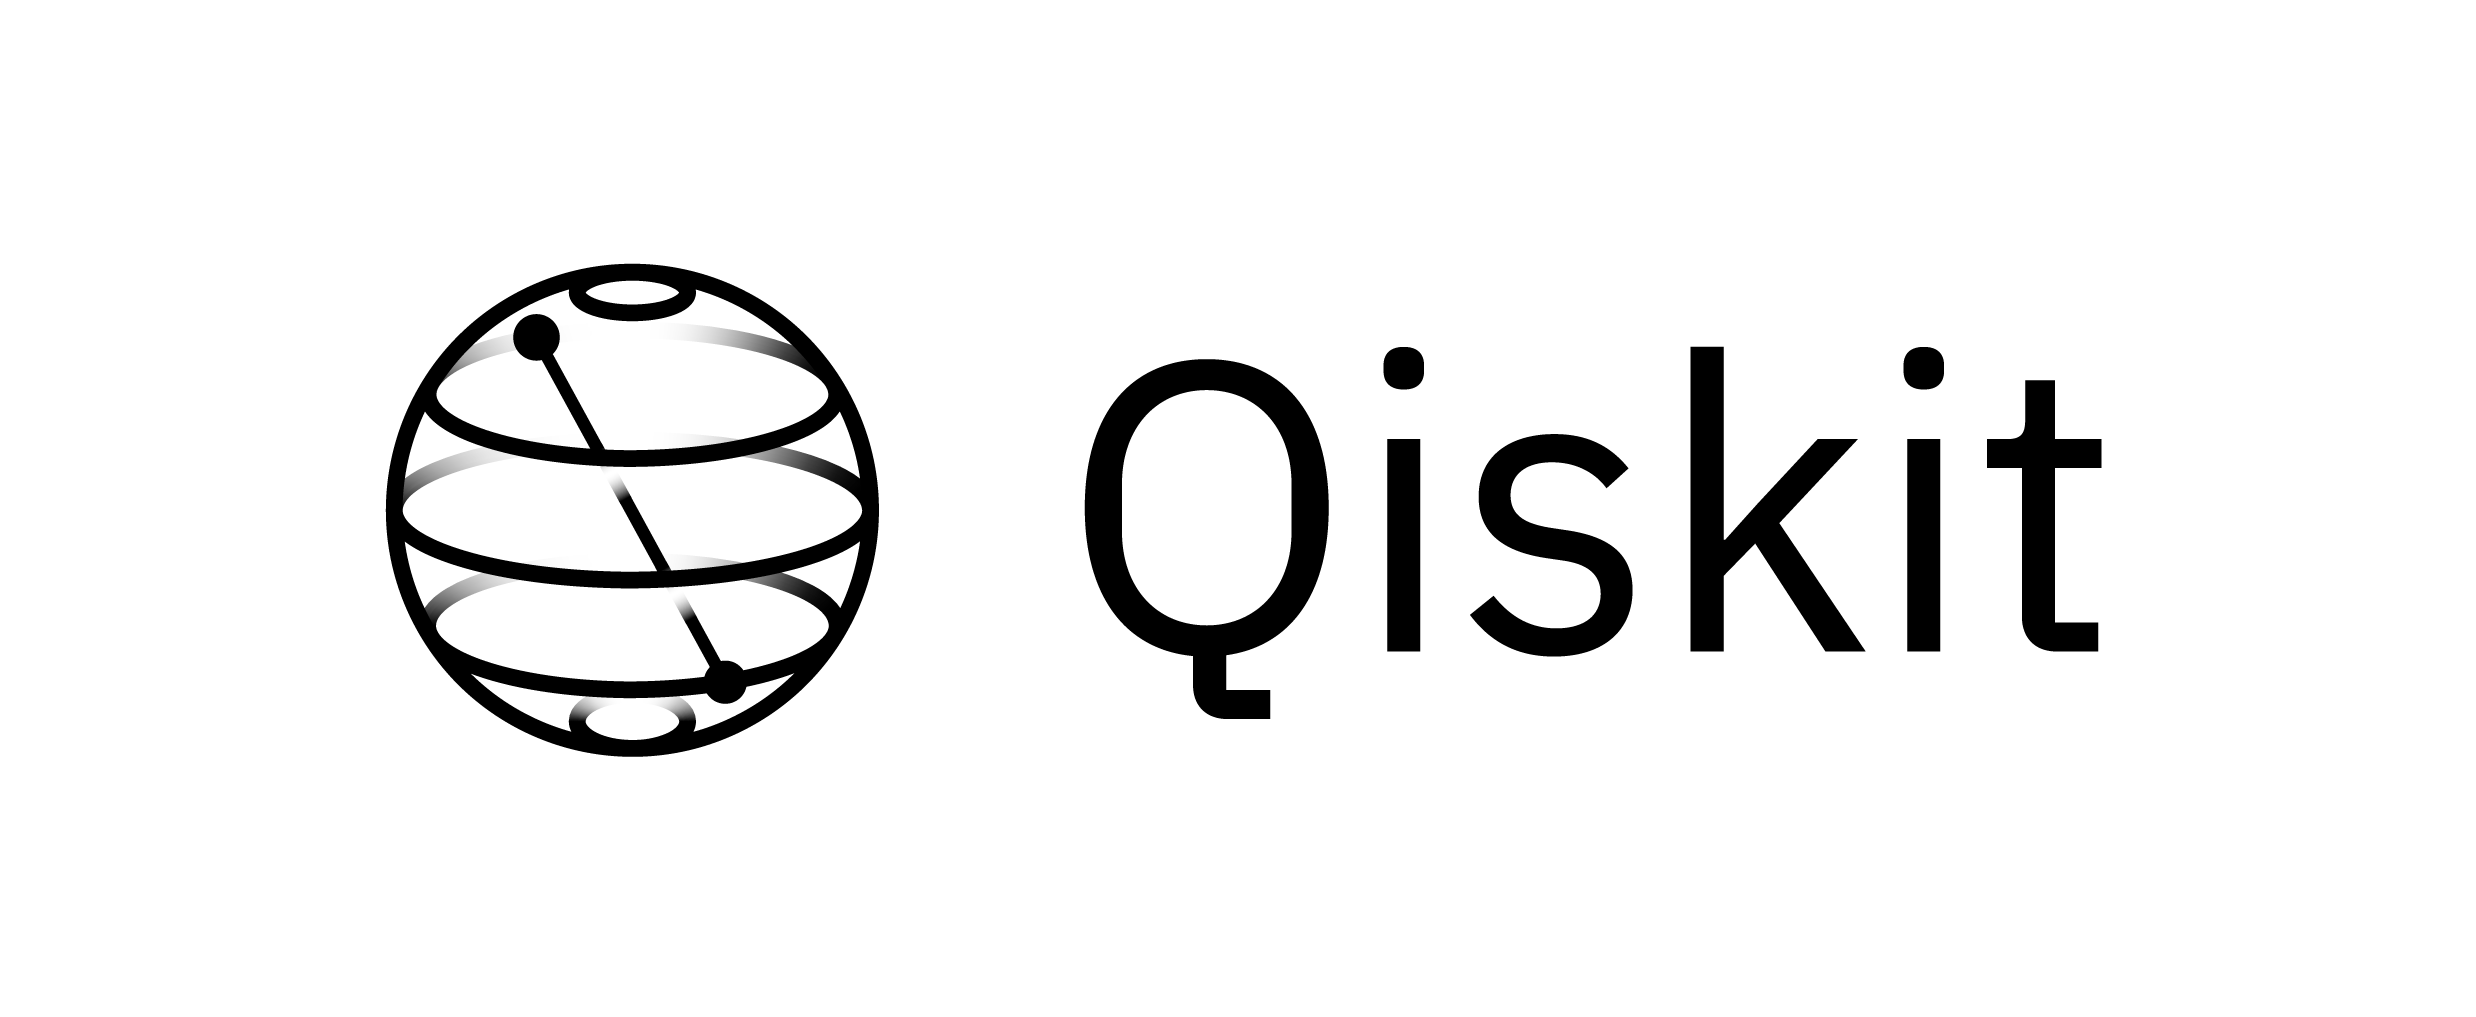
\includegraphics[scale = 0.75]{../Demonstration/img/qiskit_logo.PNG}
	\caption{The platform we used for executing the 3-SAT algorithm on a real quantum device. © Copyright 2020, Qiskit Development Team Last updated on 2020/05/14.}
\end{figure}


